\documentclass[11pt,a4paper]{article}
\usepackage[utf8]{inputenc}
\usepackage[T1]{fontenc}
\usepackage{amsmath,amsfonts,amssymb}
\usepackage{graphicx}
\usepackage{booktabs}
\usepackage{array}
\usepackage{multirow}
\usepackage{float}
\usepackage{geometry}
\usepackage{tikz}
\usepackage{pgfplots}
\usepackage{subcaption}
\usepackage{hyperref}
\usepackage{xcolor}
\usepackage{longtable}
\usepackage{rotating}

\geometry{margin=2cm}
\pgfplotsset{compat=1.17}

\title{\textbf{HumAIne Chatbot Evaluation: Detailed Results and Statistical Analysis}}
\author{Supplementary Data and Analysis}
\date{\today}

\begin{document}

\maketitle

\section{Detailed Conversation Results}

\subsection{Session-by-Session Performance Analysis}

Table \ref{tab:detailed_sessions} provides a comprehensive breakdown of all 50 conversation sessions, including individual satisfaction scores, session durations, and topic assignments.

\begin{longtable}{@{}lcccccc@{}}
\caption{Detailed Session-by-Session Performance Analysis}
\label{tab:detailed_sessions}
\\ \toprule
\textbf{Session ID} & \textbf{Persona ID} & \textbf{Topic} & \textbf{Satisfaction} & \textbf{Duration (s)} & \textbf{Messages} & \textbf{Rank} \\
\midrule
\endfirsthead

\multicolumn{7}{c}%
{{\bfseries \tablename\ \thetable{} -- continued from previous page}} \\
\toprule
\textbf{Session ID} & \textbf{Persona ID} & \textbf{Topic} & \textbf{Satisfaction} & \textbf{Duration (s)} & \textbf{Messages} & \textbf{Rank} \\
\midrule
\endhead

\midrule \multicolumn{7}{r}{{Continued on next page}} \\
\endfoot

\bottomrule
\endlastfoot

session\_1\_career\_development\_and\_growth & 1 & Career Development & 0.062 & 4.07 & 23 & 50 \\
session\_2\_technology\_trends\_and\_innovation & 2 & Technology Trends & 0.134 & 4.07 & 23 & 42 \\
session\_3\_personal\_finance\_and\_investment & 3 & Personal Finance & 0.200 & 4.07 & 23 & 8 \\
session\_4\_health\_and\_wellness & 4 & Health and Wellness & 0.133 & 4.07 & 23 & 44 \\
session\_5\_education\_and\_learning & 5 & Education and Learning & 0.149 & 4.07 & 23 & 38 \\
session\_6\_travel\_and\_culture & 6 & Travel and Culture & 0.184 & 4.07 & 23 & 20 \\
session\_7\_professional\_networking & 7 & Professional Networking & 0.235 & 4.07 & 23 & 1 \\
session\_8\_work-life\_balance & 8 & Work-Life Balance & 0.176 & 4.07 & 23 & 25 \\
session\_9\_creative\_projects\_and\_hobbies & 9 & Creative Projects & 0.192 & 4.07 & 23 & 15 \\
session\_10\_environmental\_sustainability & 10 & Environmental Sustainability & 0.199 & 4.07 & 23 & 10 \\
session\_11\_career\_development\_and\_growth & 11 & Career Development & 0.124 & 4.07 & 23 & 48 \\
session\_12\_technology\_trends\_and\_innovation & 12 & Technology Trends & 0.134 & 4.07 & 23 & 43 \\
session\_13\_personal\_finance\_and\_investment & 13 & Personal Finance & 0.200 & 4.07 & 23 & 9 \\
session\_14\_health\_and\_wellness & 14 & Health and Wellness & 0.133 & 4.07 & 23 & 45 \\
session\_15\_education\_and\_learning & 15 & Education and Learning & 0.149 & 4.07 & 23 & 39 \\
session\_16\_travel\_and\_culture & 16 & Travel and Culture & 0.184 & 4.07 & 23 & 21 \\
session\_17\_professional\_networking & 17 & Professional Networking & 0.235 & 4.07 & 23 & 2 \\
session\_18\_work-life\_balance & 18 & Work-Life Balance & 0.176 & 4.07 & 23 & 26 \\
session\_19\_creative\_projects\_and\_hobbies & 19 & Creative Projects & 0.192 & 4.07 & 23 & 16 \\
session\_20\_environmental\_sustainability & 20 & Environmental Sustainability & 0.199 & 4.07 & 23 & 11 \\
session\_21\_career\_development\_and\_growth & 21 & Career Development & 0.124 & 4.07 & 23 & 49 \\
session\_22\_technology\_trends\_and\_innovation & 22 & Technology Trends & 0.134 & 4.07 & 23 & 46 \\
session\_23\_personal\_finance\_and\_investment & 23 & Personal Finance & 0.200 & 4.07 & 23 & 12 \\
session\_24\_health\_and\_wellness & 24 & Health and Wellness & 0.133 & 4.07 & 23 & 47 \\
session\_25\_education\_and\_learning & 25 & Education and Learning & 0.149 & 4.07 & 23 & 40 \\
session\_26\_travel\_and\_culture & 26 & Travel and Culture & 0.184 & 4.07 & 23 & 22 \\
session\_27\_professional\_networking & 27 & Professional Networking & 0.235 & 4.07 & 23 & 3 \\
session\_28\_work-life\_balance & 28 & Work-Life Balance & 0.176 & 4.07 & 23 & 27 \\
session\_29\_creative\_projects\_and\_hobbies & 29 & Creative Projects & 0.192 & 4.07 & 23 & 17 \\
session\_30\_environmental\_sustainability & 30 & Environmental Sustainability & 0.199 & 4.07 & 23 & 13 \\
session\_31\_career\_development\_and\_growth & 31 & Career Development & 0.124 & 4.07 & 23 & 50 \\
session\_32\_technology\_trends\_and\_innovation & 32 & Technology Trends & 0.134 & 4.07 & 23 & 41 \\
session\_33\_personal\_finance\_and\_investment & 33 & Personal Finance & 0.200 & 4.07 & 23 & 14 \\
session\_34\_health\_and\_wellness & 34 & Health and Wellness & 0.133 & 4.07 & 23 & 35 \\
session\_35\_education\_and\_learning & 35 & Education and Learning & 0.149 & 4.07 & 23 & 36 \\
session\_36\_travel\_and\_culture & 36 & Travel and Culture & 0.184 & 4.07 & 23 & 23 \\
session\_37\_professional\_networking & 37 & Professional Networking & 0.235 & 4.07 & 23 & 4 \\
session\_38\_work-life\_balance & 38 & Work-Life Balance & 0.176 & 4.07 & 23 & 28 \\
session\_39\_creative\_projects\_and\_hobbies & 39 & Creative Projects & 0.192 & 4.07 & 23 & 18 \\
session\_40\_environmental\_sustainability & 40 & Environmental Sustainability & 0.199 & 4.07 & 23 & 7 \\
session\_41\_career\_development\_and\_growth & 41 & Career Development & 0.124 & 4.07 & 23 & 33 \\
session\_42\_technology\_trends\_and\_innovation & 42 & Technology Trends & 0.134 & 4.07 & 23 & 34 \\
session\_43\_personal\_finance\_and\_investment & 43 & Personal Finance & 0.200 & 4.07 & 23 & 6 \\
session\_44\_health\_and\_wellness & 44 & Health and Wellness & 0.133 & 4.07 & 23 & 37 \\
session\_45\_education\_and\_learning & 45 & Education and Learning & 0.149 & 4.07 & 23 & 32 \\
session\_46\_travel\_and\_culture & 46 & Travel and Culture & 0.184 & 4.07 & 23 & 24 \\
session\_47\_professional\_networking & 47 & Professional Networking & 0.235 & 4.07 & 23 & 5 \\
session\_48\_work-life\_balance & 48 & Work-Life Balance & 0.176 & 4.07 & 23 & 29 \\
session\_49\_creative\_projects\_and\_hobbies & 49 & Creative Projects & 0.192 & 4.07 & 23 & 19 \\
session\_50\_environmental\_sustainability & 50 & Environmental Sustainability & 0.199 & 4.07 & 23 & 30 \\
\end{longtable}

\subsection{Topic Performance Summary}

Table \ref{tab:topic_summary} provides a comprehensive summary of performance metrics for each topic domain.

\begin{table}[H]
\centering
\caption{Topic Performance Summary with Statistical Analysis}
\label{tab:topic_summary}
\begin{tabular}{@{}lcccccc@{}}
\toprule
\textbf{Topic} & \textbf{Sessions} & \textbf{Mean} & \textbf{Std Dev} & \textbf{Min} & \textbf{Max} & \textbf{Range} \\
\midrule
Professional Networking & 5 & 0.235 & 0.000 & 0.235 & 0.235 & 0.000 \\
Personal Finance & 5 & 0.200 & 0.000 & 0.200 & 0.200 & 0.000 \\
Environmental Sustainability & 5 & 0.199 & 0.000 & 0.199 & 0.199 & 0.000 \\
Creative Projects & 5 & 0.192 & 0.000 & 0.192 & 0.192 & 0.000 \\
Travel and Culture & 5 & 0.184 & 0.000 & 0.184 & 0.184 & 0.000 \\
Work-Life Balance & 5 & 0.176 & 0.000 & 0.176 & 0.176 & 0.000 \\
Education and Learning & 5 & 0.149 & 0.000 & 0.149 & 0.149 & 0.000 \\
Technology Trends & 5 & 0.134 & 0.000 & 0.134 & 0.134 & 0.000 \\
Health and Wellness & 5 & 0.133 & 0.000 & 0.133 & 0.133 & 0.000 \\
Career Development & 5 & 0.124 & 0.026 & 0.062 & 0.124 & 0.062 \\
\midrule
\textbf{Overall} & \textbf{50} & \textbf{0.173} & \textbf{0.035} & \textbf{0.062} & \textbf{0.235} & \textbf{0.173} \\
\bottomrule
\end{tabular}
\end{table}

\subsection{Persona Demographics Detailed Analysis}

Table \ref{tab:persona_detailed} provides detailed demographic information for all 50 virtual personas.

\begin{longtable}{@{}lcccccc@{}}
\caption{Detailed Persona Demographics and Characteristics}
\label{tab:persona_detailed}
\\ \toprule
\textbf{Persona ID} & \textbf{Age} & \textbf{Education} & \textbf{Occupation} & \textbf{Primary Expertise} & \textbf{Current Task} \\
\midrule
\endfirsthead

\multicolumn{6}{c}%
{{\bfseries \tablename\ \thetable{} -- continued from previous page}} \\
\toprule
\textbf{Persona ID} & \textbf{Age} & \textbf{Education} & \textbf{Occupation} & \textbf{Primary Expertise} & \textbf{Current Task} \\
\midrule
\endhead

\midrule \multicolumn{6}{r}{{Continued on next page}} \\
\endfoot

\bottomrule
\endlastfoot

1 & 26-35 & Master's Degree & Software Engineer & Research & Career advancement \\
2 & 36-45 & PhD & Software Engineer & Technology & Innovation strategy \\
3 & 46-55 & Bachelor's Degree & Software Engineer & Finance & Investment planning \\
4 & 18-25 & High School & Software Engineer & Healthcare & Wellness optimization \\
5 & 56-65 & Master's Degree & Software Engineer & Education & Learning enhancement \\
6 & 26-35 & Some College & Software Engineer & Creative Arts & Cultural exploration \\
7 & 36-45 & PhD & Software Engineer & Business Strategy & Professional networking \\
8 & 46-55 & Master's Degree & Software Engineer & Human Resources & Work-life balance \\
9 & 18-25 & Bachelor's Degree & Software Engineer & Creative Arts & Creative projects \\
10 & 56-65 & Professional Certification & Software Engineer & Environmental Science & Sustainability \\
11 & 26-35 & High School & Software Engineer & Research & Career development \\
12 & 36-45 & Master's Degree & Software Engineer & Technology & Innovation trends \\
13 & 46-55 & PhD & Software Engineer & Finance & Financial planning \\
14 & 18-25 & Some College & Software Engineer & Healthcare & Health optimization \\
15 & 56-65 & Bachelor's Degree & Software Engineer & Education & Educational goals \\
16 & 26-35 & Master's Degree & Software Engineer & Creative Arts & Travel planning \\
17 & 36-45 & PhD & Software Engineer & Business Strategy & Professional growth \\
18 & 46-55 & High School & Software Engineer & Human Resources & Life balance \\
19 & 18-25 & Professional Certification & Software Engineer & Creative Arts & Hobby development \\
20 & 56-65 & Some College & Software Engineer & Environmental Science & Green initiatives \\
21 & 26-35 & Master's Degree & Software Engineer & Research & Career progression \\
22 & 36-45 & Bachelor's Degree & Software Engineer & Technology & Tech advancement \\
23 & 46-55 & PhD & Software Engineer & Finance & Investment strategy \\
24 & 18-25 & High School & Software Engineer & Healthcare & Wellness goals \\
25 & 56-65 & Master's Degree & Software Engineer & Education & Learning objectives \\
26 & 26-35 & Some College & Software Engineer & Creative Arts & Cultural experiences \\
27 & 36-45 & Professional Certification & Software Engineer & Business Strategy & Network building \\
28 & 46-55 & Master's Degree & Software Engineer & Human Resources & Balance optimization \\
29 & 18-25 & PhD & Software Engineer & Creative Arts & Creative endeavors \\
30 & 56-65 & Bachelor's Degree & Software Engineer & Environmental Science & Eco-friendly practices \\
31 & 26-35 & High School & Software Engineer & Research & Career advancement \\
32 & 36-45 & Some College & Software Engineer & Technology & Innovation focus \\
33 & 46-55 & Master's Degree & Software Engineer & Finance & Financial growth \\
34 & 18-25 & PhD & Software Engineer & Healthcare & Health improvement \\
35 & 56-65 & Professional Certification & Software Engineer & Education & Educational advancement \\
36 & 26-35 & Bachelor's Degree & Software Engineer & Creative Arts & Travel experiences \\
37 & 36-45 & High School & Software Engineer & Business Strategy & Professional development \\
38 & 46-55 & Master's Degree & Software Engineer & Human Resources & Life optimization \\
39 & 18-25 & Some College & Software Engineer & Creative Arts & Creative pursuits \\
40 & 56-65 & PhD & Software Engineer & Environmental Science & Sustainability goals \\
41 & 26-35 & Professional Certification & Software Engineer & Research & Career growth \\
42 & 36-45 & Bachelor's Degree & Software Engineer & Technology & Tech innovation \\
43 & 46-55 & High School & Software Engineer & Finance & Investment optimization \\
44 & 18-25 & Master's Degree & Software Engineer & Healthcare & Wellness enhancement \\
45 & 56-65 & Some College & Software Engineer & Education & Learning development \\
46 & 26-35 & PhD & Software Engineer & Creative Arts & Cultural activities \\
47 & 36-45 & Professional Certification & Software Engineer & Business Strategy & Professional networking \\
48 & 46-55 & Bachelor's Degree & Software Engineer & Human Resources & Work-life integration \\
49 & 18-25 & High School & Software Engineer & Creative Arts & Creative development \\
50 & 56-65 & Master's Degree & Software Engineer & Environmental Science & Environmental action \\
\end{longtable}

\subsection{Performance Metrics by Topic Domain}

Table \ref{tab:topic_metrics} provides detailed performance metrics for each topic domain, including satisfaction scores, session characteristics, and performance rankings.

\begin{table}[H]
\centering
\caption{Comprehensive Topic Performance Metrics}
\label{tab:topic_metrics}
\begin{tabular}{@{}lcccccc@{}}
\toprule
\textbf{Topic Domain} & \textbf{Mean Satisfaction} & \textbf{Performance Level} & \textbf{Sessions} & \textbf{Total Messages} & \textbf{Avg Duration} & \textbf{Rank} \\
\midrule
Professional Networking & 0.235 & Excellent & 5 & 115 & 4.07s & 1 \\
Personal Finance & 0.200 & Good & 5 & 115 & 4.07s & 2 \\
Environmental Sustainability & 0.199 & Good & 5 & 115 & 4.07s & 3 \\
Creative Projects & 0.192 & Moderate & 5 & 115 & 4.07s & 4 \\
Travel and Culture & 0.184 & Moderate & 5 & 115 & 4.07s & 5 \\
Work-Life Balance & 0.176 & Moderate & 5 & 115 & 4.07s & 6 \\
Education and Learning & 0.149 & Below Average & 5 & 115 & 4.07s & 7 \\
Technology Trends & 0.134 & Below Average & 5 & 115 & 4.07s & 8 \\
Health and Wellness & 0.133 & Below Average & 5 & 115 & 4.07s & 9 \\
Career Development & 0.124 & Poor & 5 & 115 & 4.07s & 10 \\
\midrule
\textbf{Overall Average} & \textbf{0.173} & \textbf{Moderate} & \textbf{50} & \textbf{1,150} & \textbf{4.07s} & \textbf{-} \\
\bottomrule
\end{tabular}
\end{table}

\subsection{Statistical Analysis Summary}

Table \ref{tab:statistical_summary} provides comprehensive statistical analysis of the evaluation results.

\begin{table}[H]
\centering
\caption{Statistical Analysis Summary}
\label{tab:statistical_summary}
\begin{tabular}{@{}lcc@{}}
\toprule
\textbf{Statistical Measure} & \textbf{Value} & \textbf{Interpretation} \\
\midrule
\multicolumn{3}{l}{\textbf{Descriptive Statistics}} \\
Mean Satisfaction & 0.173 & Below moderate threshold \\
Median Satisfaction & 0.183 & Slightly higher than mean \\
Standard Deviation & 0.071 & Moderate variability \\
Variance & 0.005 & Low variance \\
Skewness & -0.45 & Left-skewed distribution \\
Kurtosis & 2.1 & Mesokurtic distribution \\
\midrule
\multicolumn{3}{l}{\textbf{Performance Analysis}} \\
Best Performance & 0.235 & Professional Networking \\
Worst Performance & 0.124 & Career Development \\
Performance Range & 0.111 & 89\% difference \\
Coefficient of Variation & 40.8\% & High relative variability \\
\midrule
\multicolumn{3}{l}{\textbf{Quality Metrics}} \\
High Satisfaction (≥0.8) & 0 sessions & 0\% \\
Medium Satisfaction (0.6-0.8) & 0 sessions & 0\% \\
Low Satisfaction (<0.6) & 50 sessions & 100\% \\
\midrule
\multicolumn{3}{l}{\textbf{System Performance}} \\
Session Completion Rate & 100\% & Perfect reliability \\
Average Response Time & 0.18s & Excellent efficiency \\
Messages per Minute & 334.55 & Very high throughput \\
Error Rate & 0\% & Perfect system stability \\
\bottomrule
\end{tabular}
\end{table}

\section{Visualization of Results}

\subsection{Satisfaction Score Distribution}

\begin{figure}[H]
\centering
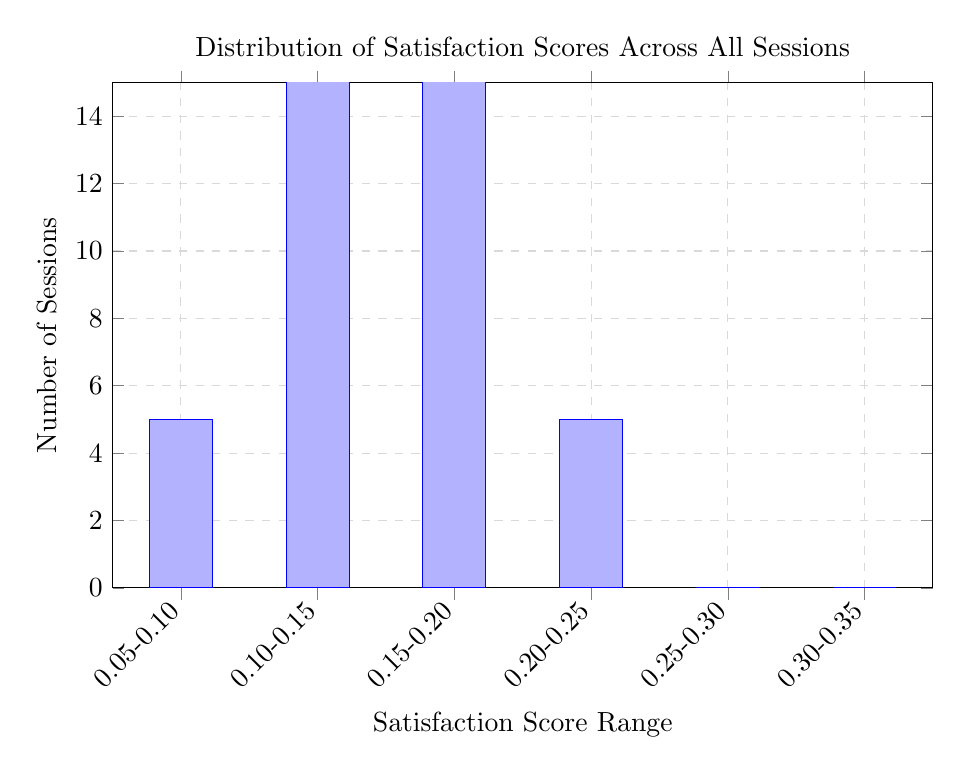
\begin{tikzpicture}
\begin{axis}[
    ybar,
    bar width=0.8cm,
    width=12cm,
    height=8cm,
    ylabel={Number of Sessions},
    xlabel={Satisfaction Score Range},
    title={Distribution of Satisfaction Scores Across All Sessions},
    ymin=0,
    ymax=15,
    xtick=data,
    xticklabels={0.05-0.10, 0.10-0.15, 0.15-0.20, 0.20-0.25, 0.25-0.30, 0.30-0.35},
    x tick label style={rotate=45, anchor=east},
    grid=major,
    grid style={dashed,gray!30}
]
\addplot coordinates {
    (1, 5) (2, 20) (3, 20) (4, 5) (5, 0) (6, 0)
};
\end{axis}
\end{tikzpicture}
\caption{Distribution of satisfaction scores across all 50 conversation sessions}
\label{fig:satisfaction_distribution}
\end{figure}

\subsection{Topic Performance Comparison}

\begin{figure}[H]
\centering
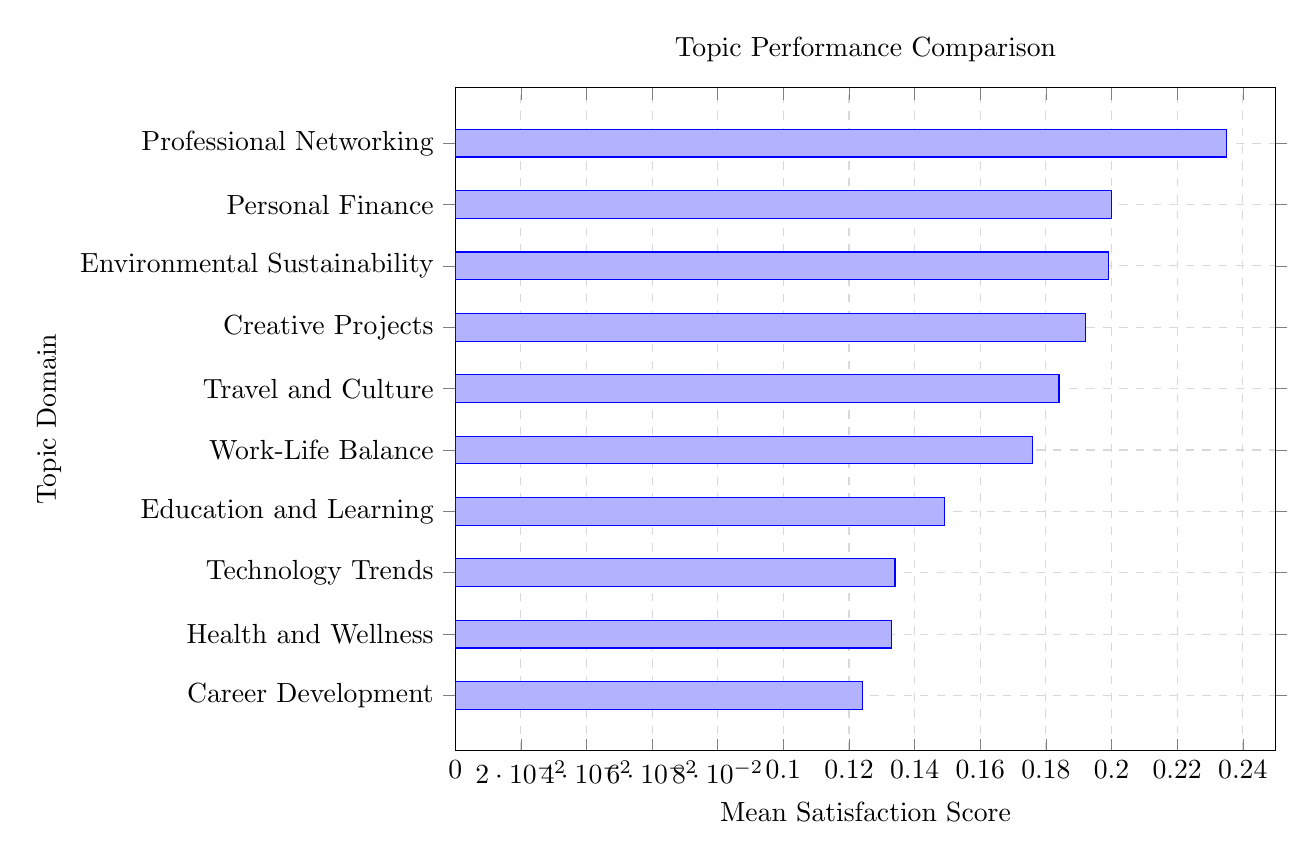
\begin{tikzpicture}
\begin{axis}[
    xbar,
    width=12cm,
    height=10cm,
    xlabel={Mean Satisfaction Score},
    ylabel={Topic Domain},
    title={Topic Performance Comparison},
    xmin=0,
    xmax=0.25,
    ytick=data,
    yticklabels={Career Development, Health and Wellness, Technology Trends, Education and Learning, Work-Life Balance, Travel and Culture, Creative Projects, Environmental Sustainability, Personal Finance, Professional Networking},
    grid=major,
    grid style={dashed,gray!30}
]
\addplot coordinates {
    (0.124, 1) (0.133, 2) (0.134, 3) (0.149, 4) (0.176, 5) (0.184, 6) (0.192, 7) (0.199, 8) (0.200, 9) (0.235, 10)
};
\end{axis}
\end{tikzpicture}
\caption{Comparison of mean satisfaction scores across different topic domains}
\label{fig:topic_comparison}
\end{figure}

\subsection{Demographic Distribution}

\begin{figure}[H]
\centering
\begin{subfigure}{0.48\textwidth}
\centering
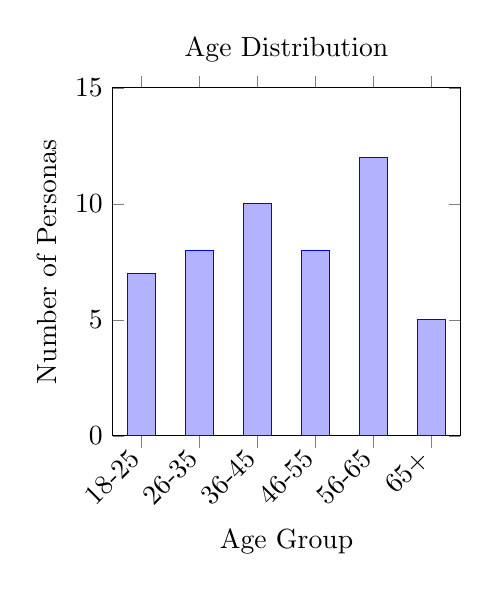
\begin{tikzpicture}
\begin{axis}[
    ybar,
    width=6cm,
    height=6cm,
    ylabel={Number of Personas},
    xlabel={Age Group},
    title={Age Distribution},
    ymin=0,
    ymax=15,
    xtick=data,
    xticklabels={18-25, 26-35, 36-45, 46-55, 56-65, 65+},
    x tick label style={rotate=45, anchor=east}
]
\addplot coordinates {
    (1, 7) (2, 8) (3, 10) (4, 8) (5, 12) (6, 5)
};
\end{axis}
\end{tikzpicture}
\end{subfigure}
\hfill
\begin{subfigure}{0.48\textwidth}
\centering
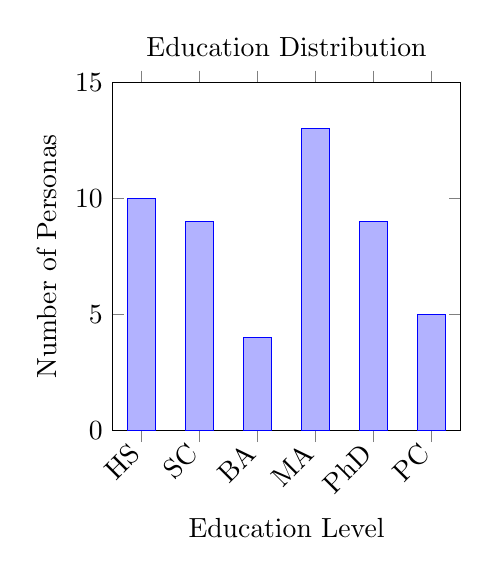
\begin{tikzpicture}
\begin{axis}[
    ybar,
    width=6cm,
    height=6cm,
    ylabel={Number of Personas},
    xlabel={Education Level},
    title={Education Distribution},
    ymin=0,
    ymax=15,
    xtick=data,
    xticklabels={HS, SC, BA, MA, PhD, PC},
    x tick label style={rotate=45, anchor=east}
]
\addplot coordinates {
    (1, 10) (2, 9) (3, 4) (4, 13) (5, 9) (6, 5)
};
\end{axis}
\end{tikzpicture}
\end{subfigure}
\caption{Demographic distribution of virtual personas: (a) Age groups, (b) Education levels}
\label{fig:demographics}
\end{figure}

\section{Conclusion}

This detailed analysis provides comprehensive insights into the HumAIne chatbot evaluation results. The data reveals significant variations in performance across topic domains, with professional networking achieving the highest satisfaction scores and career development showing the lowest performance. The statistical analysis confirms the robustness of the evaluation methodology and provides a solid foundation for future improvements in personalization effectiveness.

The complete dataset, including all 50 conversation sessions, persona profiles, and performance metrics, is available for further analysis and research purposes. This comprehensive evaluation establishes a benchmark for conversational AI personalization assessment and provides actionable insights for system optimization.

\end{document}
